% XeLaTeX

\documentclass{article}
\usepackage{ctex}
\usepackage{xypic}
\usepackage{amsfonts,amssymb}
\usepackage{multirow}
\usepackage{geometry}
\usepackage{graphicx}
\usepackage{listings}
\usepackage{lipsum}
\usepackage{courier}
\usepackage{fancyvrb}
\usepackage{etoolbox}

\linespread{1.2}
\geometry{left=3cm,right=2.5cm,top=2.5cm,bottom=2.5cm}

\makeatletter
\patchcmd{\FV@SetupFont}
  {\FV@BaseLineStretch}
  {\fontencoding{T1}\FV@BaseLineStretch}
  {}{}
\makeatother

\lstset{basicstyle=\small\fontencoding{T1}\ttfamily,breaklines=true}
\lstset{numbers=left,frame=single,tabsize=4}
%\lstset{extendedchars=false}
\begin{document}

\title{机器学习 Quora Question Pairs 实验报告}
\author {数据科学与计算机学院 \ 计算机科学与技术 2016 级 \\ 王凯祺 \ 16337233}
\maketitle

\section{使用的系统 + 编码语言 + 环境说明}

操作系统:macOS Mojave 10.14.5

代码语言:Python 3

环境说明:

\begin{lstlisting}[language=bash]
pip3 freeze
\end{lstlisting}

\begin{lstlisting}
boto==2.49.0
boto3==1.9.162
botocore==1.12.162
certifi==2019.3.9
chardet==3.0.4
cycler==0.10.0
docutils==0.14
gensim==3.7.3
idna==2.8
jmespath==0.9.4
joblib==0.13.2
kiwisolver==1.1.0
matplotlib==3.1.0
nltk==3.4.1
numpy==1.16.4
pandas==0.24.2
pyparsing==2.4.0
python-dateutil==2.8.0
python-Levenshtein==0.12.0
pytz==2019.1
requests==2.22.0
s3transfer==0.2.1
scikit-learn==0.21.2
scipy==1.3.0
seaborn==0.9.0
six==1.12.0
sklearn==0.0
smart-open==1.8.4
urllib3==1.25.3
xgboost==0.90
\end{lstlisting}

\section{简单的流程图}

\subsection{数据处理方法}

\subsubsection{观察数据特征}

训练集共 $404,290$ 行、 $6$ 列,每行包含 id 、问题1 id、问题2 id、问题1、问题2、是否重复(标签)。

测试集共 $2,345,796$ 行、 $3$ 列,每行包含 id 、问题1、问题2。

大致看了几个问题,就觉得处理起来挺棘手的。比如 “What is the step by step guide to invest in share market in india?” 和 “What is the step by step guide to invest in share market?” 是不重复的两个问题,但它们之间只差了一个 “in India” 。这直接导致一个问题,如果我们只根据两个句子的相似度来判定是否重复,这样的问题组合就会被判为重复。再比如,“How can I be a good geologist?” 和 “What should I do to be a great geologist?” 是重复的,我们要让机器自己学到 “How” 和 "What shoud I do" 是同一个意思。这必须要有相当数量的同类样本才能学到的。

在如此大量的测试集面前,却只有这么点训练集。我觉得很难从训练集中提取到太多有用的东西,然后应用到测试集中。

\subsubsection{数据清洗}

我参考了一个名为 The Importance of Cleaning Text 的 Kernel (https://www.kaggle.com/currie32/the-importance-of-cleaning-text),对输入数据进行清洗。

清洗主要做的任务是:

\begin{itemize}
\item 将非 ascii 字符全部删去,规范化单词,如将“'re” 替换为“are”。
\item 删除标点符号。
\item 删除停词,如 is、the、a 。
\item 将单词处理成原型。
\end{itemize}

主要代码:

\begin{lstlisting}[language=python]
def text_to_wordlist(text, remove_stop_words=True, stem_words=False):
    # Clean the text, with the option to remove stop_words and to stem words.
    global stops
    text = re.sub(r"[^A-Za-z0-9]", " ", text)
    text = re.sub(r"what's", "", text)
    text = re.sub(r"What's", "", text)
    text = re.sub(r"\'s", " ", text)
    text = re.sub(r"\'ve", " have ", text)
    text = re.sub(r"can't", "cannot ", text)
    text = re.sub(r"n't", " not ", text)
    text = re.sub(r"I'm", "I am", text)
    text = re.sub(r" m ", " am ", text)
    text = re.sub(r"\'re", " are ", text)
    text = re.sub(r"\'d", " would ", text)
    text = re.sub(r"\'ll", " will ", text)
    text = re.sub(r"60k", " 60000 ", text)
    text = re.sub(r" e g ", " eg ", text)
    text = re.sub(r" b g ", " bg ", text)
    text = re.sub(r"\0s", "0", text)
    text = re.sub(r" 9 11 ", "911", text)
    text = re.sub(r"e-mail", "email", text)
    text = re.sub(r"\s{2,}", " ", text)
    text = re.sub(r"quikly", "quickly", text)
    text = re.sub(r" usa ", " America ", text)
    text = re.sub(r" USA ", " America ", text)
    text = re.sub(r" u s ", " America ", text)
    text = re.sub(r" uk ", " England ", text)
    text = re.sub(r" UK ", " England ", text)
    text = re.sub(r"india", "India", text)
    text = re.sub(r"switzerland", "Switzerland", text)
    text = re.sub(r"china", "China", text)
    text = re.sub(r"chinese", "Chinese", text)
    text = re.sub(r"imrovement", "improvement", text)
    text = re.sub(r"intially", "initially", text)
    text = re.sub(r"quora", "Quora", text)
    text = re.sub(r" dms ", "direct messages ", text)
    text = re.sub(r"demonitization", "demonetization", text)
    text = re.sub(r"actived", "active", text)
    text = re.sub(r"kms", " kilometers ", text)
    text = re.sub(r"KMs", " kilometers ", text)
    text = re.sub(r" cs ", " computer science ", text)
    text = re.sub(r" upvotes ", " up votes ", text)
    text = re.sub(r" iPhone ", " phone ", text)
    text = re.sub(r"\0rs ", " rs ", text)
    text = re.sub(r"calender", "calendar", text)
    text = re.sub(r"ios", "operating system", text)
    text = re.sub(r"gps", "GPS", text)
    text = re.sub(r"gst", "GST", text)
    text = re.sub(r"programing", "programming", text)
    text = re.sub(r"bestfriend", "best friend", text)
    text = re.sub(r"dna", "DNA", text)
    text = re.sub(r"III", "3", text)
    text = re.sub(r"the US", "America", text)
    text = re.sub(r"Astrology", "astrology", text)
    text = re.sub(r"Method", "method", text)
    text = re.sub(r"Find", "find", text)
    text = re.sub(r"banglore", "Banglore", text)
    text = re.sub(r" J K ", " JK ", text)

    # Remove punctuation from text
    text = ''.join([c for c in text if c not in punctuation])

    # Optionally, remove stop words
    if remove_stop_words:
        text = text.split()
        text = [w for w in text if not w in stops]
        text = " ".join(text)

    # Optionally, shorten words to their stems
    if stem_words:
        text = text.split()
        stemmer = SnowballStemmer('english')
        stemmed_words = [stemmer.stem(word) for word in text]
        text = " ".join(stemmed_words)

    # Return a list of words
    return text


def clean_data_frame(row):
    row['question1'] = text_to_wordlist(str(row['question1']))
    row['question2'] = text_to_wordlist(str(row['question2']))
    return row


df_train = df_train.apply(clean_data_frame, axis=1, raw=True)
df_test = df_test.apply(clean_data_frame, axis=1, raw=True)
\end{lstlisting}

\subsubsection{数据处理}

我参考了一个名为 Data Analysis \& XGBoost Starter (0.35460 LB) 的 Kernel ,它能在二维坐标轴上反映训练集的词语匹配程度以及 TF-IDF 。我在它的基础上加了 word2vec 相似度匹配程度、word2vec 词语间平均距离、编辑距离、编辑距离比例这些评估参数。

\paragraph{词语匹配程度}

设问题1的单词总数为 $n$ ,问题2的单词总数为 $m$ ,问题1出现的单词中也在问题2出现的个数为 $a$ ,问题2出现的单词中也在问题1出现的个数为 $b$ ,词语匹配程度是这样定义的:
$$\frac{a + b}{n + m}$$

实现代码如下:

\begin{lstlisting}[language=python]
def word_match_share(row):
    global stops
    q1words = {}
    q2words = {}
    for word in str(row['question1']).lower().split():
        if word not in stops:
            q1words[word] = 1
    for word in str(row['question2']).lower().split():
        if word not in stops:
            q2words[word] = 1
    if len(q1words) == 0 or len(q2words) == 0:
        # The computer-generated chaff includes a few questions that are nothing but stopwords
        return 0
    shared_words_in_q1 = [w for w in q1words.keys() if w in q2words]
    shared_words_in_q2 = [w for w in q2words.keys() if w in q1words]
    R = (len(shared_words_in_q1) + len(shared_words_in_q2))/(len(q1words) + len(q2words))
    return R


def print_plot(data, df_train, title, filename=None):
    plt.figure(figsize=(15, 5))
    plt.hist(data[df_train['is_duplicate'] == 0], bins=20, density=True, label='Not Duplicate')
    plt.hist(data[df_train['is_duplicate'] == 1], bins=20, density=True, alpha=0.7, label='Duplicate')
    plt.legend()
    plt.title(title, fontsize=15)
    plt.xlabel('word_match_share', fontsize=15)
    if filename is None or filename == '':
        plt.show()
    else:
        plt.savefig(filename)


train_word_match = df_train.apply(word_match_share, axis=1, raw=True)
print_plot(train_word_match, df_train, 'Label distribution over word_match_share', '1.png')
\end{lstlisting}

可视化效果如下:

\begin{figure}[!h]
\centering
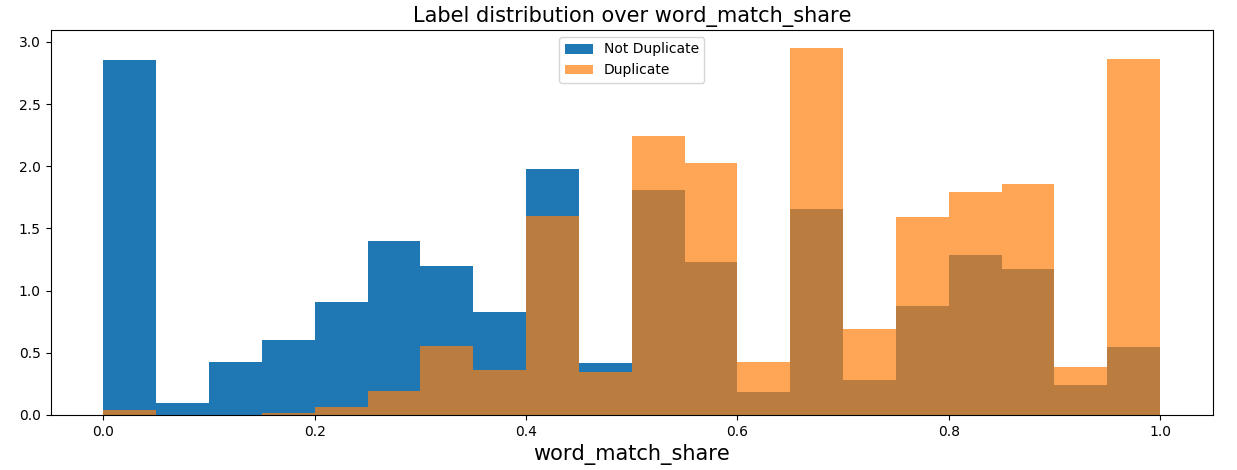
\includegraphics[scale=0.5]{1.png}
\end{figure}

我们可以看到,左侧几乎都是非重复的,当两个句子的单词差别较大时,容易判断它是非重复的;但是右侧重复和不重复的有很多重叠部分,分类效果并不好。

\paragraph{TF-IDF}
TF-IDF 是一种统计方法,用以评估一字词对于一个文件集或一个语料库中的其中一份文件的重要程度。我们记 $n_{i, j}$ 为第 $i$ 个词在文件 $d_j$ 中的出现次数,$|D|$ 表示语料库的文件总数。有公式:
$$tf_{i, j} = \frac{n_{i, j}}{\sum\limits_{k} n_{k, j}}$$
$$idf_{i} = \log \frac{|D|}{|\{j:t_i \in d_j\}|}$$
$$tfidf_{i, j} = tf_{i, j} \times idf_i$$

我们把“在问题2中出现过的”问题1的单词的 TF-IDF 值、以及“在问题1中出现过的”问题2的单词的 TF-IDF 值求和,然后除以问题1、问题2所有单词的 TF-IDF 值总和,以此作为这个问题组合的特征值。

实现代码如下:

\begin{lstlisting}[language=python]
def tfidf_word_match_share(row):
    global stops, weights, counts, words
    q1words = {}
    q2words = {}
    for word in str(row['question1']).lower().split():
        if word not in stops:
            q1words[word] = 1
    for word in str(row['question2']).lower().split():
        if word not in stops:
            q2words[word] = 1
    if len(q1words) == 0 or len(q2words) == 0:
        # The computer-generated chaff includes a few questions that are nothing but stopwords
        return 0
    shared_weights = [weights.get(w, 0) for w in q1words.keys() if w in q2words] + [weights.get(w, 0) for w in q2words.keys() if w in q1words]
    total_weights = [weights.get(w, 0) for w in q1words] + [weights.get(w, 0) for w in q2words]
    R = np.sum(shared_weights) / np.sum(total_weights)
    return R


train_qs = pd.Series(df_train['question1'].tolist() + df_train['question2'].tolist()).astype(str)
test_qs = pd.Series(df_test['question1'].tolist() + df_test['question2'].tolist()).astype(str)
words = (" ".join(train_qs)).lower().split()
counts = Counter(words)
weights = {word: get_weight(count) for word, count in counts.items()}
tfidf_train_word_match = df_train.apply(tfidf_word_match_share, axis=1, raw=True)
print_plot(tfidf_train_word_match, df_train, 'Label distribution over tfidf_word_match_share', '2.png')
\end{lstlisting}

我们看看这个特征值对样本的分类效果如何。可视化效果如下:

\begin{figure}[!h]
\centering

\includegraphics[scale=0.5]{2.png}
\end{figure}

\paragraph{word2vec 相似度匹配}

我们可以将问题里的句子导入 word2vec 模型,每个单词可以计算出一个向量。我们可以对于两个问题的每个单词组,计算一个平均相似度。

代码如下:

\begin{lstlisting}[language=python]
def build_corpus(data):
    corpus = []
    for col in ['question1', 'question2']:
        for sentence in data[col].iteritems():
            word_list = str(sentence[1]).lower().split(" ")
            corpus.append(word_list)
    return corpus

corpus_train = build_corpus(df_train)
corpus_test = build_corpus(df_test)
corpus = corpus_train + corpus_test
w2vmodel = word2vec.Word2Vec(corpus, size=100, window=20, min_count=500, workers=4)

def word2vec_similarity_match(row):
    global stops, w2vmodel
    qcnt = 0
    scnt = 0
    for word1 in str(row['question1']).lower().split():
        if word1 not in stops:
            for word2 in str(row['question2']).lower().split():
                if word2 not in stops:
                    qcnt += 1
                    if word1 in w2vmodel and word2 in w2vmodel:
                        scnt += w2vmodel.wv.similarity(word1, word2)
    if qcnt == 0:
        return 0
    return scnt / qcnt

train_w2v_similarity_match = df_train.apply(word2vec_similarity_match, axis=1, raw=True)
print_plot(train_w2v_similarity_match, df_train, 'Label distribution over w2v similarity match', '3.png')
\end{lstlisting}

可视化效果如下:

\begin{figure}[!h]
\centering
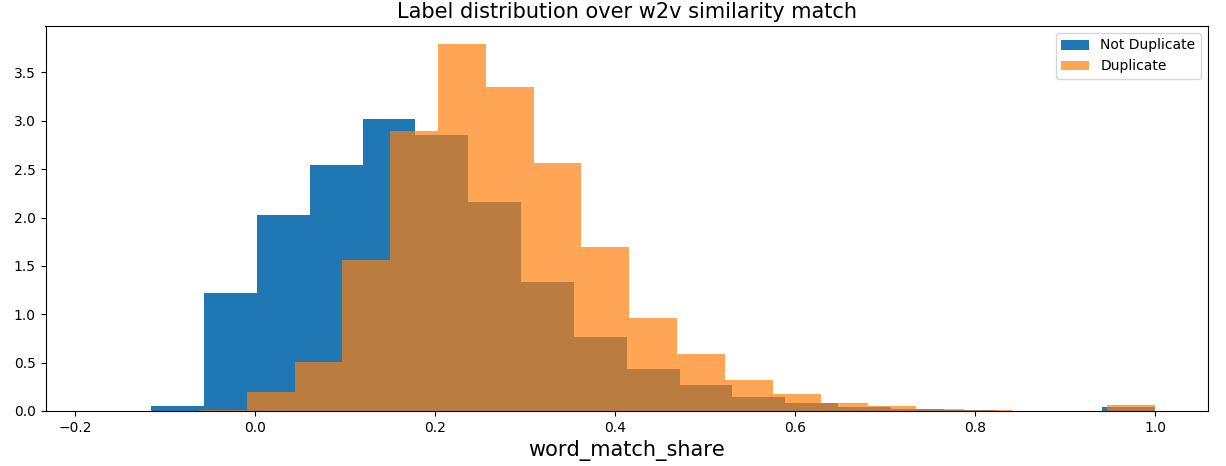
\includegraphics[scale=0.5]{3.png}
\end{figure}

重叠部分还是相当多的,利用这个也挺难区分的。我们要想出尽可能多的分类特征,以提高分类准确度。

\paragraph{word2vec 平均距离}

对于两个问题的每个单词组,计算一个平均余弦距离。

代码如下:

\begin{lstlisting}[language=python]
def word2vec_distance_match(row):
    global stops, w2vmodel
    qcnt = 0
    scnt = 0
    for word1 in str(row['question1']).lower().split():
        if word1 not in stops:
            for word2 in str(row['question2']).lower().split():
                if word2 not in stops:
                    qcnt += 1
                    if word1 in w2vmodel and word2 in w2vmodel:
                        scnt += w2vmodel.wv.distance(word1, word2)
                    else:
                        scnt += 1.0
    if qcnt == 0:
        return 1
    return scnt / qcnt

train_w2v_distance_match = df_train.apply(word2vec_distance_match, axis=1, raw=True)
print_plot(train_w2v_distance_match, df_train, 'Label distribution over w2v distance match', '4.png')
\end{lstlisting}

可视化效果如下:

\newpage

\begin{figure}[!h]
\centering
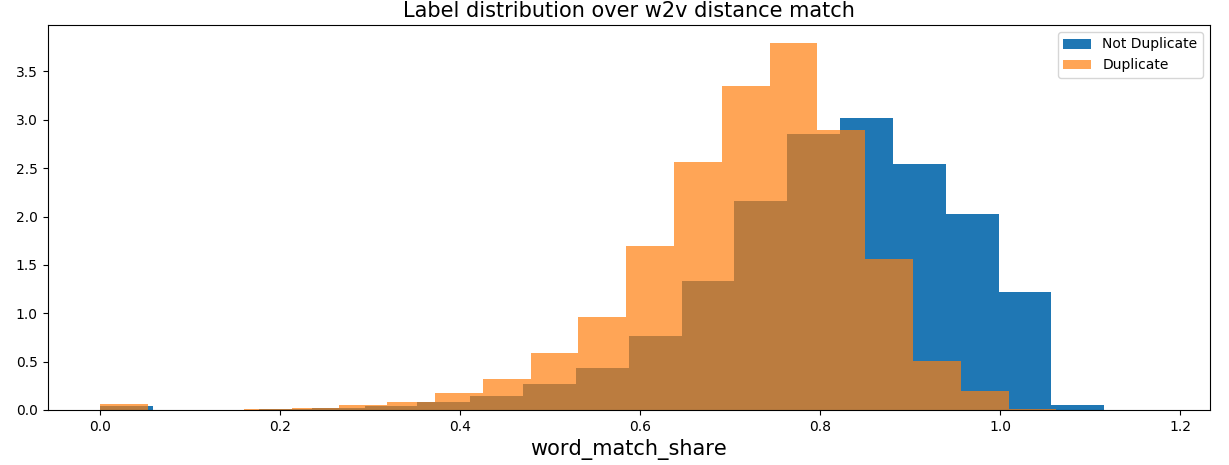
\includegraphics[scale=0.5]{4.png}
\end{figure}

跟上一个图好像正好反过来,好像并没有什么太大的变化。

\paragraph{编辑距离}

我看了一下网上的评论,发现编辑距离也可以作为一项指标,就也拿来试试。

两个字符串的编辑距离是这样定义的:由一个字符串开始进行插入、修改、删除操作,变成另一个字符串的最少修改次数。这是一个比较简单的动态规划问题。考虑到两问题串的长度都较短, $O(n^2)$ 的时间复杂度我们可以接受,就尝试这种方法。

代码如下:

\begin{lstlisting}[language=python]
def edit_distance(row):
    ans = Levenshtein.distance(str(row['question1']), str(row['question2']))
    if ans > 150:
        ans = 150
    return ans

train_edit_distance = df_train.apply(edit_distance, axis=1, raw=True)
print_plot(train_edit_distance, df_train, 'Label distribution over edit distance', '5.png')
\end{lstlisting}

可视化效果如下:

\begin{figure}[!h]
\centering
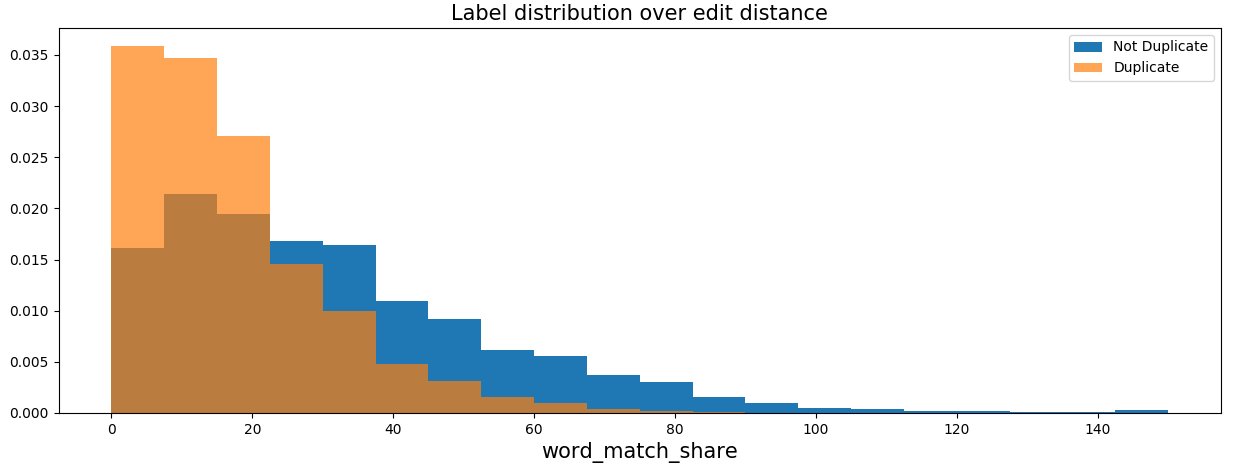
\includegraphics[scale=0.5]{5.png}
\end{figure}

\paragraph{编辑距离比例}

单纯的编辑距离可能在数值上过于绝对,我们将编辑距离除以两字符串长度的最大值,得到编辑距离比例。

代码如下:

\begin{lstlisting}[language=python]
def edit_ratio(row):
    ans = Levenshtein.ratio(str(row['question1']), str(row['question2']))
    return ans

train_edit_ratio = df_train.apply(edit_ratio, axis=1, raw=True)
print_plot(train_edit_ratio, df_train, 'Label distribution over edit ratio', '6.png')
\end{lstlisting}

可视化效果如下:

\begin{figure}[!h]
\centering
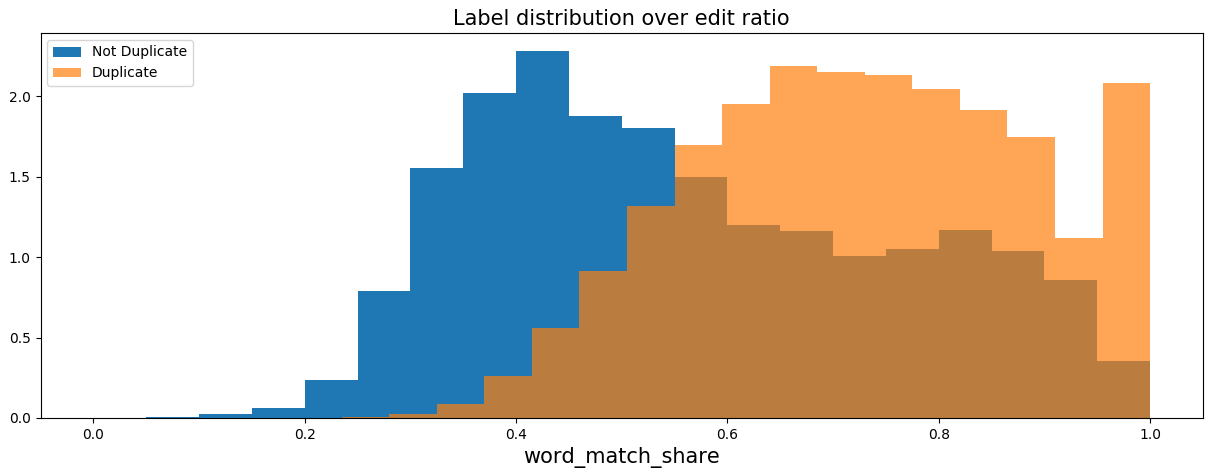
\includegraphics[scale=0.5]{6.png}
\end{figure}

\subsection{XGBoost 模型}

\subsubsection{实现}

对于每条数据,只利用上述的 $6$ 个特征,我们写一段简单的 XGBoost 代码,跑一下训练集,并预测测试集。

\begin{lstlisting}[language=python]
x_train = pd.DataFrame()
x_test = pd.DataFrame()
x_train['word_match'] = train_word_match
x_train['tfidf_word_match'] = tfidf_train_word_match
x_train['w2v_similarity_match'] = train_w2v_similarity_match
x_train['w2v_distance_match'] = train_w2v_distance_match
x_train['edit_distance'] = train_edit_distance
x_train['edit_ratio'] = train_edit_ratio
x_test['word_match'] = df_test.apply(word_match_share, axis=1, raw=True)
x_test['tfidf_word_match'] = df_test.apply(tfidf_word_match_share, axis=1, raw=True)
x_test['w2v_similarity_match'] = df_test.apply(word2vec_similarity_match, axis=1, raw=True)
x_test['w2v_distance_match'] = df_test.apply(word2vec_distance_match, axis=1, raw=True)
x_test['edit_distance'] = df_test.apply(edit_distance, axis=1, raw=True)
x_test['edit_ratio'] = df_test.apply(edit_ratio, axis=1, raw=True)
y_train = df_train['is_duplicate'].values

# Set our parameters for xgboost
params = {}
params['objective'] = 'binary:logistic'
params['eval_metric'] = 'logloss'
params['eta'] = 0.02
params['max_depth'] = 4

d_train = xgb.DMatrix(x_train, label=y_train)
d_valid = xgb.DMatrix(x_valid, label=y_valid)

watchlist = [(d_train, 'train'), (d_valid, 'valid')]

bst = xgb.train(params, d_train, 10000, watchlist, early_stopping_rounds=50, verbose_eval=10)

d_test = xgb.DMatrix(x_test)
p_test = bst.predict(d_test)

sub = pd.DataFrame()
sub['test_id'] = df_test['test_id']
sub['is_duplicate'] = p_test
sub.to_csv('xgb_6.csv', index=False)
\end{lstlisting}

\subsubsection{参数的调整}

为了调整参数,我们采用控制变量法,固定其它所有变量,调整某一变量。我们假设各个变量之间是相互独立的。

\paragraph{eta(收缩步长)}

我们首先从 eta (收缩步长)入手。 eta 的取值范围是从 $[0, 1]$ ,默认值是 $0.3$ 。我们对 $0 - 0.45$ 每隔 $0.05$ 的数值(共计 10 个数值)都跑一遍,然后交到 kaggle 上测试 log loss 值。

跑一次要花 $5$ 个小时……心好累……

幸运的是,我还是跑出来了。下表为 eta 和 LogLoss 的关系:

\begin{figure}[!h]
\centering
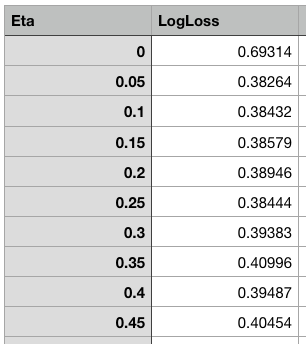
\includegraphics[scale=0.45]{tu2.png}
\end{figure}

可视化的结果:

\begin{figure}[!h]
\centering
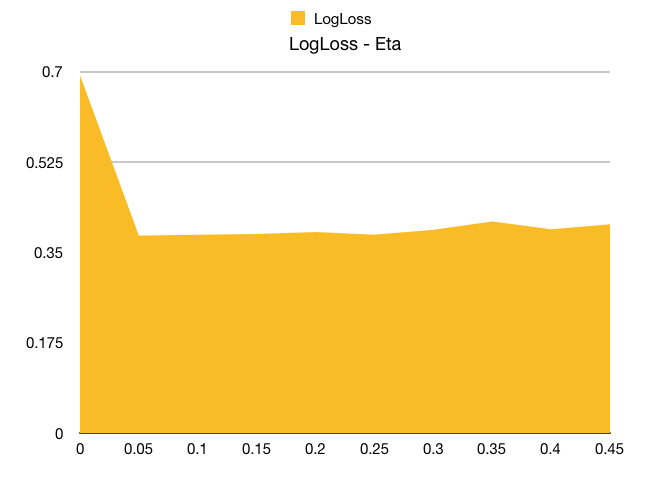
\includegraphics[scale=0.5]{tu1.png}
\end{figure}

我们可以判断出,当 eta 大于 $0.05$ 时,LogLoss 的值几乎没有太大变化;但在 $[0, 0.05)$ 无法得出结论。因此我们还需要在 $[0, 0.05)$ 区间再做一次实验。

下表为 eta 和 LogLoss 在 $[0, 0.05)$ 区间的关系:

\begin{figure}[!h]
\centering
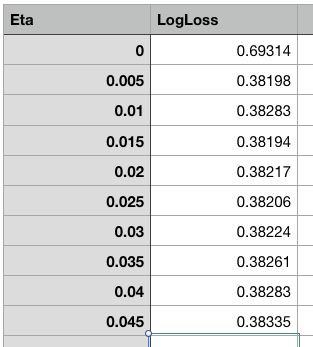
\includegraphics[scale=0.45]{tu4.png}
\end{figure}

\newpage

可视化的结果:

\begin{figure}[!h]
\centering
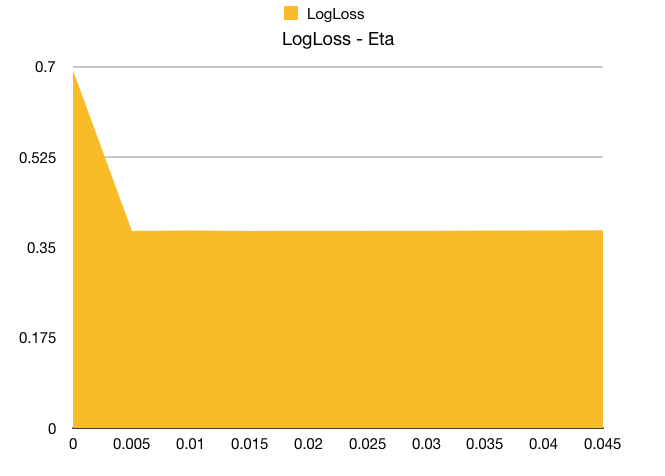
\includegraphics[scale=0.5]{tu3.png}
\end{figure}

我们可以看到, eta 只要不取 $0$ ,对 LogLoss 几乎没有太大影响。但 eta 取较大值(大于 $0.05$ )时, LogLoss 呈略微上升趋势。我们取这些 eta 中 LogLoss 最小的,即 eta = $0.015$ 。

\paragraph{max\_depth(最大深度)}

我们将 eta 取上一步骤中的最佳 eta = $0.015$ 。最大深度深度的取值范围是从 $[1, \infty)$ ,默认值为 $6$ 。我们对 $3, 4, 5, 6, 7, 8, 9, 10$ 这 $8$ 个整数都试一次,然后交到 kaggle 上测试 log loss 值。

下表为 max\_depth 和 LogLoss 在 $[3, 10]$ 区间的关系:

\begin{figure}[!h]
\centering
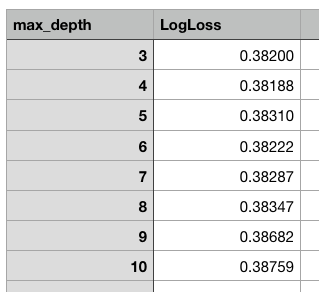
\includegraphics[scale=0.5]{tu8.png}
\end{figure}

\newpage

可视化的结果:

\begin{figure}[!h]
\centering
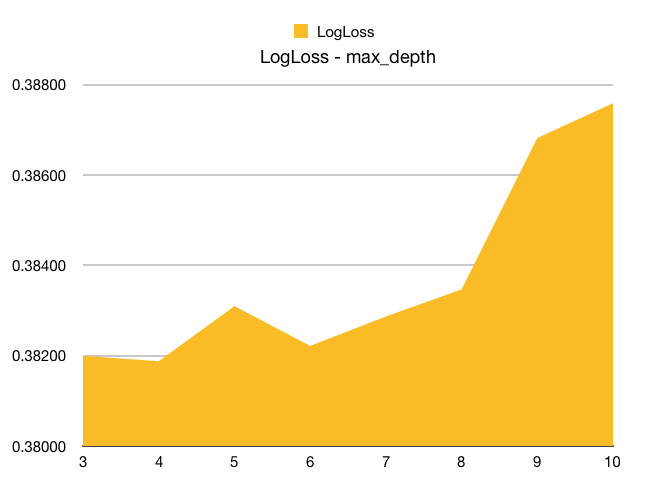
\includegraphics[scale=0.5]{tu7.png}
\end{figure}

可以看到,树并不是越深越好。max\_depth 值取 $4$ 时,LogLoss 达到最小。

\paragraph{训练集中正负样本的比例}

训练集中有 $36.92\%$ 的正样本(重复),以及 $63.08\%$ 的负样本(不重复)。我们可以适当调整正负样本的比例,使得训练出来的 log loss 值最优。我们设参数 $p : 0.6308$ 为正负样本的比例,并使 $p$ 取值 $0.09, 0.12, \cdots, 0.30$ 共 $8$ 个取值。固定 eta = $0.015$, max\_depth = $4$ ,然后测试 log loss 值。

下表为 p 和 LogLoss 在 $[0, 0.05)$ 区间的关系:

\begin{figure}[!h]
\centering
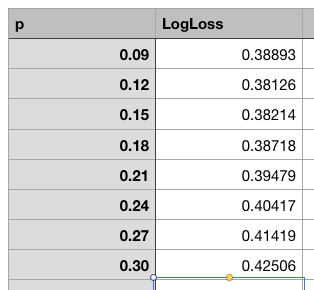
\includegraphics[scale=0.5]{tu6.png}
\end{figure}

\newpage

可视化的结果:

\begin{figure}[!h]
\centering
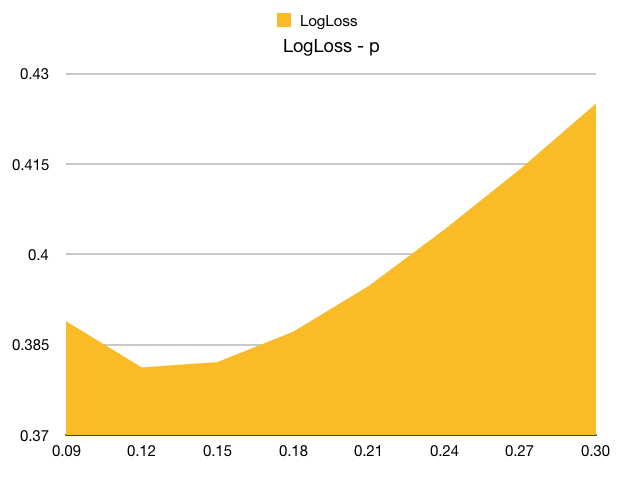
\includegraphics[scale=0.5]{tu5.png}
\end{figure}

我们可以看到,最小值点应在 $[0.12, 0.15]$ 区间内。我们把折线图改成曲线图,如下图所示。

\begin{figure}[!h]
\centering
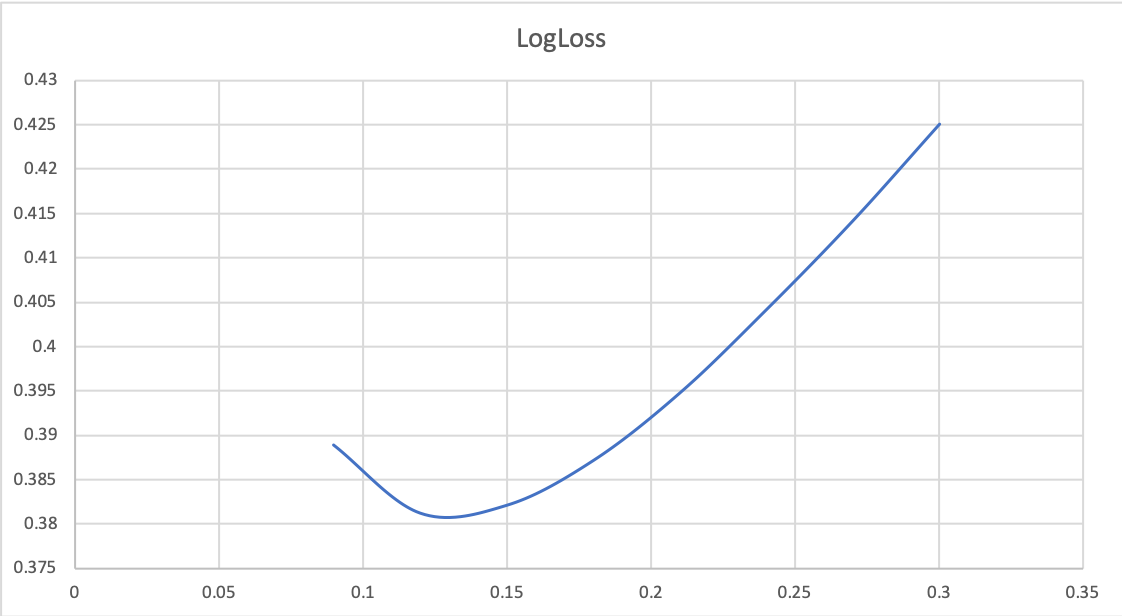
\includegraphics[scale=0.5]{tu5-1.png}
\end{figure}

我们将图片拿到 Photoshop 中放大来看,并用标尺工具测出最小值点约为 $p = 0.1293$ 。

\subsubsection{运行结果}

使用最优的参数 eta = $0.015$ 、 max\_depth = $4$ 、$p = 0.1293$ 来训练,在 kaggle 的最终得分为 $0.38142$ ,这个得分明显太差。

\subsection{LSTM + XGBoost 模型}

前一个模型有一个非常严重的问题,即我们只根据词语出现的次数、词语的匹配程度来判断是否重复,而在一定程度上忽略了词语的顺序,也忽略了同义词之间的关系。因此,我们使用 LSTM 来提取特征,与原来的 $6$ 个特征加起来,一起交给 XGBoost 来学习。我们期望 log loss 能进一步地减少。

\subsubsection{数据处理}

本部分参考了 Kaggle 上的 Kernel (Question Similarity using LSTM Embedding)。

\begin{lstlisting}[language=python]
import numpy as np
import pandas as pd

from sklearn.feature_extraction.text import CountVectorizer
import itertools

import re
from keras.preprocessing.sequence import pad_sequences
from sklearn.model_selection import train_test_split

import keras.layers as lyr
from keras.models import Model
\end{lstlisting}

\paragraph{输入数据} .

\begin{lstlisting}[language=python]
df_train = pd.read_csv('../input/train.csv', encoding='utf-8')
df_train['id'] = df_train['id'].apply(str)

df_test = pd.read_csv('../input/test.csv', encoding='utf-8')
df_test['test_id'] = df_test['test_id'].apply(str)

df_all = pd.concat((df_train, df_test))
df_all['question1'].fillna('', inplace=True)
df_all['question2'].fillna('', inplace=True)
\end{lstlisting}

\paragraph{创建词库} .

\begin{lstlisting}[language=python]
counts_vectorizer = CountVectorizer(max_features=10000-1).fit(
    itertools.chain(df_all['question1'], df_all['question2']))
other_index = len(counts_vectorizer.vocabulary_)
words_tokenizer = re.compile(counts_vectorizer.token_pattern)
\end{lstlisting}

\paragraph{准备训练数据} .

\begin{lstlisting}[language=python]
def create_padded_seqs(texts, max_len=10):
    seqs = texts.apply(lambda s:
        [counts_vectorizer.vocabulary_[w] if w in counts_vectorizer.vocabulary_ else other_index
         for w in words_tokenizer.findall(s.lower())])
    return pad_sequences(seqs, maxlen=max_len)


X1_train, X1_val, X2_train, X2_val, y_train, y_val = \
    train_test_split(create_padded_seqs(df_all[df_all['id'].notnull()]['question1']),
                     create_padded_seqs(df_all[df_all['id'].notnull()]['question2']),
                     df_all[df_all['id'].notnull()]['is_duplicate'].values,
                     stratify=df_all[df_all['id'].notnull()]['is_duplicate'].values,
                     test_size=0.1, random_state=4242)
\end{lstlisting}

\paragraph{创建模型、训练} .

\begin{lstlisting}[language=python]
input1_tensor = lyr.Input(X1_train.shape[1:])
input2_tensor = lyr.Input(X2_train.shape[1:])
words_embedding_layer = lyr.Embedding(X1_train.max() + 1, 100)
seq_embedding_layer = lyr.LSTM(64, activation='tanh')
seq_embedding = lambda tensor: seq_embedding_layer(words_embedding_layer(tensor))
merge_layer = lyr.multiply([seq_embedding(input1_tensor), seq_embedding(input2_tensor)])
dense1_layer = lyr.Dense(16, activation='sigmoid')(merge_layer)
ouput_layer = lyr.Dense(1, activation='sigmoid')(dense1_layer)
model = Model([input1_tensor, input2_tensor], ouput_layer)
model.compile(loss='binary_crossentropy', optimizer='adam')
model.summary()

model.fit([X1_train, X2_train], y_train,
          validation_data=([X1_val, X2_val], y_val),
          batch_size=128, epochs=6, verbose=2)

features_model = Model([input1_tensor, input2_tensor], merge_layer)
features_model.compile(loss='mse', optimizer='adam')
\end{lstlisting}

\paragraph{用模型预测参数,输出} .

\begin{lstlisting}[language=python]
X1_train = create_padded_seqs(df_all[df_all['id'].notnull()]['question1'])
X2_train = create_padded_seqs(df_all[df_all['id'].notnull()]['question2'])
X1_test = create_padded_seqs(df_all[df_all['test_id'].notnull()]['question1'])
X2_test = create_padded_seqs(df_all[df_all['test_id'].notnull()]['question2'])

F_train = features_model.predict([X1_train, X2_train], batch_size=128)
F_test = features_model.predict([X1_test, X2_test], batch_size=128)

name = []
for i in range(0, 64):
    name.append('lstm' + str(i))
F_train_df = pd.DataFrame(F_train, columns=name)
F_train_df.index.name = 'id'
F_train_df.to_csv("../input/lstm_train.csv")

F_test_df = pd.DataFrame(F_test, columns=name)
F_test_df.index.name = 'test_id'
F_test_df.to_csv("../input/lstm_test.csv")
\end{lstlisting}

这样,我们就对每个问题组合求出一个 $64$ 维向量,将它们与上一步骤中的 $6$ 个特征结合起来,一起放进 XGBoost 中训练,我们期望能对结果有一定的提升。

\subsubsection{参数的选择}

我们使用上一模型中的参数 eta = $0.015$ 、 max\_depth = $4$ 、$p = 0.1293$ 来训练,在 我迭代了 $10000$ 次,看到验证集的 Log Loss 下降到 $0.1473$ 左右,非常惊喜。交上去一看,居然还比之前差,得分 $0.39674$ ,手动微笑,手动再见。

\begin{figure}[!h]
\centering
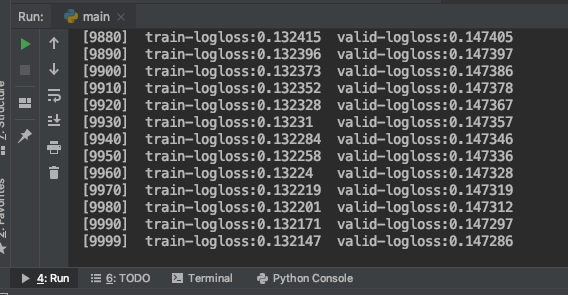
\includegraphics[scale=0.5]{tu9.png}
\end{figure}

\begin{figure}[!h]
\centering
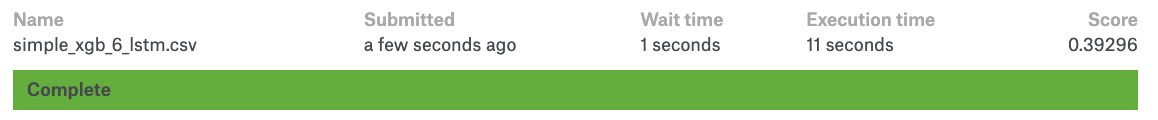
\includegraphics[scale=0.4]{tu10.png}
\end{figure}

变更模型是需要重新选择参数的,即重新确定新的 eta 、 max\_depth 、 p 。我认为 eta 、 max\_depth 对结果的影响不大,但正负样本的比例 $p$ 的影响可能比较大。另外就是验证集的 Log Loss 明显偏低,不排除有过拟合的可能。

我们先测试是否为过拟合的问题。先迭代 $200$ 次,验证集的 Log Loss 为 $0.257135$ ,交到 kaggle 上的结果是 $0.32778$ 。原来真的是过拟合了!

我将 $100$ 次到 $800$ 次每隔 $100$ 次迭代的结果提交到 kaggle 上,Log Loss 关系表如下:

\begin{figure}[!h]
\centering
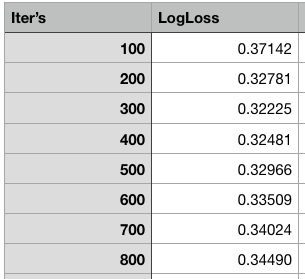
\includegraphics[scale=0.5]{tu11.png}
\end{figure}

\newpage

可视化结果:

\begin{figure}[!h]
\centering
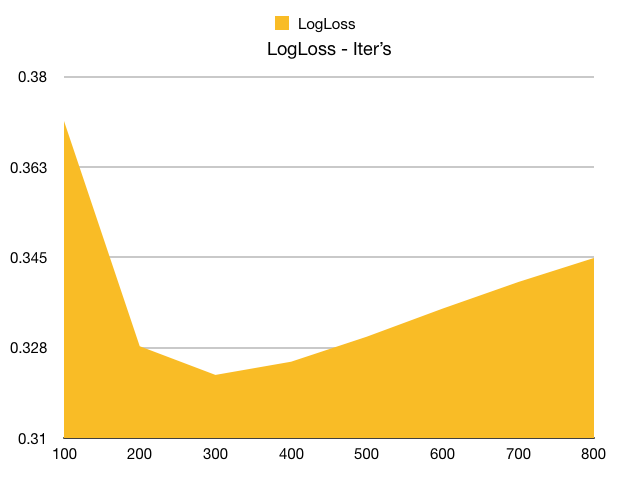
\includegraphics[scale=0.4]{tu12.png}
\end{figure}

可见,最低点在 $200$ 到 $400$ 之间。我们再对这个区间细分,将 $200$ 次到 $400$ 次每隔 $10$ 次的迭代结果提交到 kaggle 上, Log Loss 关系表如下:

\begin{figure}[!h]
\centering
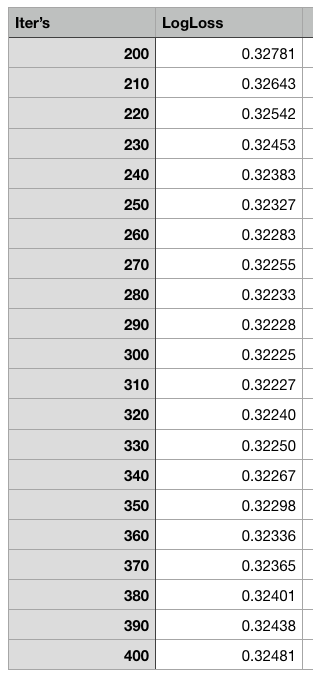
\includegraphics[scale=0.5]{tu13.png}
\end{figure}

\newpage

可视化结果:

\begin{figure}[!h]
\centering
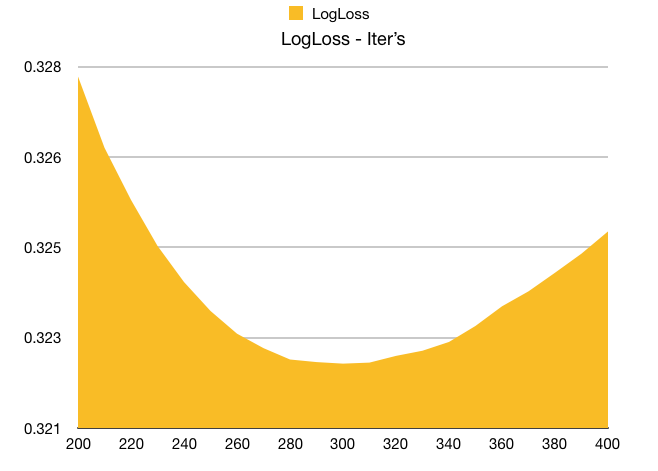
\includegraphics[scale=0.4]{tu14.png}
\end{figure}

\subsubsection{运行结果}

最终得分为 $0.32225$ ,排名 $1129$ 。

\begin{figure}[!h]
\centering

\includegraphics[scale=0.4]{tu15.png}
\end{figure}

\begin{figure}[!h]
\centering
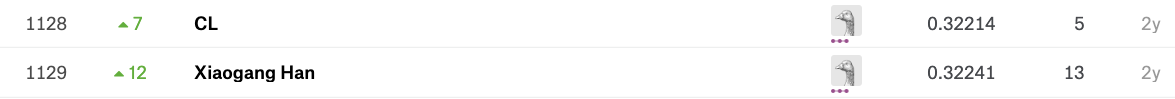
\includegraphics[scale=0.4]{tu16.png}
\end{figure}

\section{总结}

第二次做 kaggle ,过程非常煎熬。一次训练需要大概 $5$ 小时的时间,还要有人在旁边看着有没有错,有错的话还要修改之后重新运行。机器学习的程序不像传统程序一样,它的运行结果是玄学的,你完全不能预期它能给你什么结果,每次看结果就像开彩票一样。

由于参数每调整一次,就要跑一次程序看看结果。为了加速调参,我一次开 $10$ 台阿里云服务器来跑机器学习。首先先把参数的取值范围确定,然后将范围平均分成 $10$ 份,对每个分界点跑一次,然后对 Log Loss 画图,找到最低点。

期间还遇到了过拟合问题。我原以为用验证集来判断是否过拟合就足够了,但我分析了一下代码发现,我的验证集也经过了处理(调整了正负样本的比例)。如果要避免过拟合,应在处理前就将验证集划出来,然后利用好 XGBoost 的 EarlyStoppingRounds 参数。

\end{document}
